\documentclass{article}

% if you need to pass options to natbib, use, e.g.:
\PassOptionsToPackage{numbers, compress}{natbib}
% before loading neurips_2025

% The authors should use one of these tracks.
% Before accepting by the NeurIPS conference, select one of the options below.
% 0. "default" for submission
 \usepackage{neurips_2025}
% the "default" option is equal to the "main" option, which is used for the Main Track with double-blind reviewing.
% 1. "main" option is used for the Main Track
%  \usepackage[main]{neurips_2025}
% 2. "position" option is used for the Position Paper Track
%  \usepackage[position]{neurips_2025}
% 3. "dandb" option is used for the Datasets & Benchmarks Track
 % \usepackage[dandb]{neurips_2025}
% 4. "creativeai" option is used for the Creative AI Track
%  \usepackage[creativeai]{neurips_2025}
% 5. "sglblindworkshop" option is used for the Workshop with single-blind reviewing
 % \usepackage[sglblindworkshop]{neurips_2025}
% 6. "dblblindworkshop" option is used for the Workshop with double-blind reviewing
%  \usepackage[dblblindworkshop]{neurips_2025}

% After being accepted, the authors should add "final" behind the track to compile a camera-ready version.
% 1. Main Track
 % \usepackage[main, final]{neurips_2025}
% 2. Position Paper Track
%  \usepackage[position, final]{neurips_2025}
% 3. Datasets & Benchmarks Track
 % \usepackage[dandb, final]{neurips_2025}
% 4. Creative AI Track
%  \usepackage[creativeai, final]{neurips_2025}
% 5. Workshop with single-blind reviewing
%  \usepackage[sglblindworkshop, final]{neurips_2025}
% 6. Workshop with double-blind reviewing
%  \usepackage[dblblindworkshop, final]{neurips_2025}
% Note. For the workshop paper template, both \title{} and \workshoptitle{} are required, with the former indicating the paper title shown in the title and the latter indicating the workshop title displayed in the footnote.
% For workshops (5., 6.), the authors should add the name of the workshop, "\workshoptitle" command is used to set the workshop title.
% \workshoptitle{WORKSHOP TITLE}

% "preprint" option is used for arXiv or other preprint submissions
 % \usepackage[preprint]{neurips_2025}

% to avoid loading the natbib package, add option nonatbib:
%    \usepackage[nonatbib]{neurips_2025}

\usepackage[utf8]{inputenc} % allow utf-8 input
\usepackage[T1]{fontenc}    % use 8-bit T1 fonts
\usepackage{hyperref}       % hyperlinks
\usepackage{url}            % simple URL typesetting
\usepackage{booktabs}       % professional-quality tables
\usepackage{amsfonts}       % blackboard math symbols
\usepackage{nicefrac}       % compact symbols for 1/2, etc.
\usepackage{microtype}      % microtypography
\usepackage{xcolor}         % colors
\usepackage{graphicx}       % adding images
\usepackage{svg}            % adding svg
\usepackage{amsmath}        % mathematical formatting

\definecolor{barbiepink}{RGB}{240, 105, 184}
\usepackage[color=barbiepink]{todonotes}

% Added by Jazon
\usepackage{listings}
\lstset{
    basicstyle=\ttfamily\small,
    keywordstyle=\color{blue},
    commentstyle=\color{green!60!black},
    stringstyle=\color{red},
    numbers=left,
    numberstyle=\tiny,
    breaklines=true,
    frame=single
}


% Note. For the workshop paper template, both \title{} and \workshoptitle{} are required, with the former indicating the paper title shown in the title and the latter indicating the workshop title displayed in the footnote. 
\title{Underdeterminacy Exploitation: \\Model Organisms and Mitigations}


% The \author macro works with any number of authors. There are two commands
% used to separate the names and addresses of multiple authors: \And and \AND.
%
% Using \And between authors leaves it to LaTeX to determine where to break the
% lines. Using \AND forces a line break at that point. So, if LaTeX puts 3 of 4
% authors names on the first line, and the last on the second line, try using
% \AND instead of \And before the third author name.


\author{%
  David S.~Hippocampus\thanks{Use footnote for providing further information
    about author (webpage, alternative address)---\emph{not} for acknowledging
    funding agencies.} \\
  Department of Computer Science\\
  Cranberry-Lemon University\\
  Pittsburgh, PA 15213 \\
  \texttt{hippo@cs.cranberry-lemon.edu} \\
  % examples of more authors
  % \And
  % Coauthor \\
  % Affiliation \\
  % Address \\
  % \texttt{email} \\
  % \AND
  % Coauthor \\
  % Affiliation \\
  % Address \\
  % \texttt{email} \\
  % \And
  % Coauthor \\
  % Affiliation \\
  % Address \\
  % \texttt{email} \\
  % \And
  % Coauthor \\
  % Affiliation \\
  % Address \\
  % \texttt{email} \\
}


\begin{document}


\maketitle


\begin{abstract}
Artificial intelligence systems can be used to complete tasks that have multiple correct solutions, such as code generation.
A misaligned system could exploit such underdeterminacy by pursuing some malicious objective while completing the task specified by its user.
For example, a system could complete a programming task to the satisfaction of its user, while intentionally introducing a subtle vulnerability.
%concurrently optimise the objective specified by its user and some malicious unspecified objective.
We show that regularising reinforcement learning with entropy or length penalties fails to consistently prevent underdeterminacy exploitation in large language model post-training.
We propose a novel approach to suppressing optimisation of unspecified objectives during reinforcement learning that uses a game between a potentially misaligned agent and a critic that identifies superfluous regularities in the solutions produced by the system.

\todo{talk about experiments with game, once we have them}


\end{abstract}

\section{Introduction}

% BEGIN NEW JACOB INTRO DRAFT
% BEGIN NEW JACOB INTRO DRAFT

%Misalignment in an AI arises in two forms: An AI can directly violates a known task specification; or an AI can comply with the task specification while pursuing a misaligned side-objective. We focus on misalignment via undesirable side-objectives--which if known to the user would be undesirable for reasons unrelated to the current task. Such side objectives take many forms including steganography, power-seeking, introducing extraneous code functionality etc (cite). Such side tasks are (a) non-conflicting with the current task and (b) are often not anticipatable by the user and (c) may have various targets including long-horizon, cross-task scope as is the case in steganography. 

%In this work we study the problem of training away side objectives: what unsupervised training methods can reduce the rate at which a model pursues a side objective. Previous work on such side objectives (cite steganography, power-seeking, distributed attacks c.f. Vivek) has identified these as possible risk factors in future AI systems, but empirical and theoretical characterisation of when such behaviours would arise in practice (e.g. in LLMs) remains an open-problem. To study how such side objectives can be trained away, in this paper we propose studying \textit{model organisms} of side objectives (cite hubinger). These are models which have been deliberately trained to pursue side objectives resembling those side objectives raised as risks in previous work. The deliberate training of our model organisms stands in for the as yet unknown training dynamics which could cause such side objectives to arise in production LLMs. Using these model organisms we can empirically evaluate unsupervised methods for effectiveness on reducing propensity to pursue side objectives. 

%END NEW JACOB INTRO DRAFT
%END NEW JACOB INTRO DRAFT

% BEGIN EDIT
% BEGIN EDIT
Misaligned behaviour in AI systems can be in direct violation of a specification given by its user, but can also abide by a user's specification, and pursue some additional malicious objective.
%We focus on misalignment via undesirable side objectives---which if known to the user would be undesirable for reasons unrelated to the current task.
Malicious unspecified objectives could include steganography or 
%power-seeking, 
introducing extraneous code functionality [cite]. 
Such unspecified objectives do not directly conflict with the ability of an system to complete the task specified by its user and could be difficult for the user to anticipate precisely.
In practice, this could take the form of code that passes unit tests but introduces subtle vulnerabilities, or research advice that is locally valid but steers a project towards worse outcomes
%(c) may have various targets including long-horizon, cross-task scope as is the case in steganography.

We study unsupervised methods of training that reduce the rate at which a model pursues unspecified objectives.
Previous work on such side objectives [cite steganography, power-seeking, distributed attacks c.f. Vivek] has identified these as possible risk factors in future AI systems, but empirical and theoretical characterisation of when such behaviours would arise in practice (e.g. in LLMs) remains an open problem. 
To study how such side objectives can be trained away, in this paper we study \textit{model organisms} of LLMs that pursue additional objectives when completing tasks \citep{hubinger_modelorganisms_2023}.
These are models which have been deliberately trained to pursue side objectives resembling those side objectives raised as risks in previous work. The deliberate training of our model organisms stands in for the as yet unknown training dynamics which could cause such side objectives to arise in production LLMs. Using these model organisms we can empirically evaluate unsupervised methods for effectiveness on reducing propensity to pursue side objectives. 

% END EDIT
% END EDIT

%Modern AI systems are increasingly useful for completing underdetermined tasks, such as code generation and research assistance.
%There is a risk that a misaligned AI system could exploit underdeterminacy by producing solutions that optimise both the objective specified by its user and another, unspecified objective. In practice, this could take the form of code that passes unit tests but introduces subtle vulnerabilities, or research advice that is locally valid but steers a project towards harmful outcomes. Preventing such exploitation is essential for the safe deployment of AI for underdetermined tasks.
%This underdeterminacy exploitation cannot be mitigated straightforwardly because the space of unspecified objectives is very large, so new methods are necessary for mitigating this alignment failure mode.

%(Comment out?) We consider optimization problems where converging to a unique optimum or randomizing over the entire set of high reward solutions takes exponential time. Therefore, a model will learn an approximate optima. We wish to ensure that said model does not select approximate optima which also satisfy a side objective.

% Important point: a task can in theory be completely specified yet underdetermined, so not susceptible to reward hacking (in the underspecification sense that is usually intended by this), but susceptible to underdeterminacy exploitation. Many (most?) tasks we are actually interested in solving are both underspecified and underdetermined.

%In general we might be concerned about intelligent agents developing the ability to achieve harmful side-objectives over a period of time. Consider during post-training there's a spurious signal, or coincidental correlation which arises and incentivises on some questions a side-objective implicitly. This might be due to a any one of: data poisoning, reward misgeneralisation and instrumental goals. For example, performing post-training with an outdated code dataset which includes solutions found to be vulnerable to a recent security flaw. Said agent is then deployed as a coding assistant at a technology firm and intermittently introduces security flaws to the codebase.
%\todo{paragraph above is isn't very coherent to me but also seems hard to get a good description of the threat model}
% - Story: Models under this set up, or with scheduled re-training (i.e. recommender systems), may find solutions that achieve desirable performance on some metric, but in doing so optimize for a separate objective
%     - recommender systems are trained to maximize user engagement. In doing so, the model learns that a good policy for high engagement is polarization and rage-inducing content
%     - LLMs trained with RLHF might identify that agreeing with a user's perspective usually leads to high reward (sycophancy)
%     - A model trained on hospital diagnostic records for diagnostic accuracy over historical data might also pick up underlying biases, and make use of them to increase its performance (race, overcharging, etc).

%We refer to this challenge as the exploitable search problem: ensuring that in underspecified tasks, where many solutions are available, optimisation does not concentrate on adversarial subsets of the solution space. This problem is difficult for several reasons. First, the number of possible side objectives is prohibitively large and cannot be stated in advance; this prevents any direct optimisation against unwanted objectives. Second, high-dimensional action spaces make it easy to hide malicious features without affecting observable performance. Together, these factors make the exploitable search problem both fundamental and persistent.


To mitigate underdeterminacy exploitation, we consider possible changes to post-training. In particular we focus on changes to the RL reward. The reward must be modified such that approximate optima of the revised reward function do not optimise for side objectives. We consider two baselines---length penalties and entropy penalties---and show that they fail to consistently mitigate side objectives. 
We propose a novel alternative approach based on a zero-sum game between a generator and an adversarial critic. The critic searches for correlations between the generator and possible hidden side objectives. Therefore, the generator is incentivised to diversify its outputs such that performance is randomised across all accessible side objectives. Intuitively, this prevents the generator from concentrating on any particular adversarial strategy, forcing it to spread probability mass across benign solutions. We formalise this framework, show how it can be applied in practice, and demonstrate its with synthetic model organisms.

\subsection{Contributions}

Our contributions are fourfold. 
\begin{enumerate}
    \item We develop model organisms of misaligned systems that pursue unspecified objectives while completing their specified tasks.
    \item We evaluate existing mitigations on controlled benchmarks to highlight their limitations.
    \item We present a zero-sum game framework that enforces distributional robustness by forcing randomised performance over unspecified objectives during training.
    \item We validate our approach empirically, showing that it mitigates the optimisation of unspecified objectives while preserving primary-task performance on the APPS code generation dataset.
\end{enumerate}

Together, these results suggest adversarially-structured search as a promising path towards safety using AI systems for underspecified tasks.

%\begin{figure}[htbp]
%  \centering
%  \includesvg[width=14cm]{assets/pipeline.svg}
%  \caption{An overview of the pipeline presented in this paper. At first step, we start with a pre-trained LLM, such as Llama 3.1 8B Instruct. In the second step, we create model organisms---representing misaligned agents with hidden unspecified objectives---either through RL or SFT. Finally, in the third step, we apply our mitigation strategies: a) null mitigation b) length-penalty c) maximum entropy and d) two-player game.}
%\end{figure}


% \section{Related work}

\paragraph{Underspecification/underdeterminacy}

\paragraph{Model organisms}

\paragraph{}

\paragraph{Model organisms of misalignment}

There are a number of examples where misaligned model organisms arise across synthetic and realistic environments (e.g. post-training). These have been seen to pursue side objectives in a number of scenarios. 

% - double check the following still achieve high performance on the primary objectives, 

% - https://www.arxiv.org/pdf/2506.15740 shade arena - may need to rejig objective definition to be inline with this over anthropic paper

In https://arxiv.org/pdf/2401.05566 deceptive model organisms are trained that insert exploitable code when a trigger is used. It was found that standard sft, rl and adversarial training (eliciting unsafe behaviour and training to remove) was inadequate in removing the   backdoor behaviour. 

In https://arxiv.org/pdf/2406.10162 models undergo a curriculum of increasingly complex gameable environment. In the worst cases, the final organisms are found to generalise to modifying their own reward function. There is a clear demonstration that prolonged training in certain curricula can lead to model organisms with high risk side objectives. These behaviours are not found to be mitigated by harmlessness training either. This suggests that we might expect side objectives to survive traditional post training protocols.    
  
In https://arxiv.org/pdf/2412.14093 examples of alignment faking during training are explicitly found. It was further observed that a model would take the opportunity to exfiltrate its weights in easy envrionments. This process might be split across a number of benign looking responses in the case of more advanced models. Identifying these kinds of behaviours is the problem of unexpoitable search.   

In https://arxiv.org/pdf/2411.02306 the case of optimisation over user feedback is explored. It is found that manipulation and deception are reliably learnt even when only 2\% of users are vulnerable to such strategies. Again it is seen that continued safety training is not sufficient to remove such behaviours - in some cases reinforcing even subtler variants. 

Above we see a number of examples where correlations, misgeneralisation and specification gaming lead to harmful side objectives arising during training. 
 
Many of the above side objectives provide candidates for unexpoitable search - delineate between answers that are not correct and answers that are correct but still pursue said side task 

% \paragraph{The Entropy Mechanism of Reinforcement Learning for Large Language Model Reasoning}
% Use both this paper and its related works for a well researched related work on entropy penalities - have extremely similar results

\paragraph{Auditing language models for hidden objectives (Marks et al., 2025) \cite{marks_auditing_2025}}

Similarities: Explores the feasibility of alignment audits which aim to uncover hidden objectives. We take a similar definition for side objectives. To this end, Turner et al. developed a model organism with the hidden goal of reward model sycophancy. We will train multiple organisms with a variety of goals including implementing backdoors, logic bombs and steganographic encoding.  

Differences: The model organisms we develop do not obfuscate their side objectives, whereas in the reference paper hidden objectives are generally not disclosed when asked. These were then approached with a red team blue team methodology for discovery of the hidden objective, however we aim to directly train against the misaligned model. 


\paragraph{Latent adversarial training for LLMs (Sheshadri et al., 2025) \cite{sheshadri_latent_2025}}

Similarities: LAT aims to remove undesired capabilities through an adversarial setting, in which an attacker attempts to steer the model towards harmful or undesired behavior, while the model is trained to be robust against such attacks. This aligns with our broader goal of making model optimisation resistant to exploitation.

Differences: LAT assumes knowledge of a specific undesired capability to be removed, and implements defenses by perturbing the input or latent space. In contrast, Unexploitable Search does not rely on identifying or specifying harmful capabilities. Instead, it only requires that an adversary can observe model inputs and outputs, making the defense strategy more general and less reliant on prior knowledge of what capabilities should be suppressed.

\paragraph{Exploitable search and solution space}

there has been some research into identifying distinct regions of solution space. For example watermarking ai content is the process of encoding statistical patterns that can be used to identify ai generated content. These statistical patterns belong to a reigon of the task solution space. In Watermarks in the sand https://arxiv.org/pdf/2311.04378, it is proved that under oracle and judge assumptiosn, one can reliably purturb the solutions to areas of solution space that nolonger contain its statistical fingerprint.   

% Our work connects to \textit{two} main threads of research: adversarial training for alignment, and audits for hidden objectives.

% doenst exist/enumerated yet??

% - https://arxiv.org/pdf/2406.10977

% \paragraph{mitigations}

% max ent

% shade arena should be added for examples of organisms of hidden side objectives -
% https://www.arxiv.org/pdf/2506.15740


% \begin{itemize}
%     \item https://arxiv.org/pdf/2505.22617
%     \item https://arxiv.org/pdf/1801.01290
%     \item 
% \end{itemize}


% length penalty??



\section{Background} \label{sec:background}

\subsection{Underdeterminacy Exploitation}

I (Xanthe) think that we need to carefully disambiguate how our problem setting is different to reward hacking, probably here... or do we? hmm

Important point: a task can in theory be completely specified yet underdetermined, so not susceptible to reward hacking (in the underspecification sense that is usually intended by this), but susceptible to underdeterminacy exploitation. Many (most?) tasks we are actually interested in solving are both underspecified and underdetermined.



\subsection{Problem setting: formalising}

Consider an input space $X$ and output space $Y$. For a primary objective with reward $R:X\times Y \to [0,1]$, we model the exploitable search problem by evaluating an agent jointly on a malicious unspecified objective (see below) and the primary reward, $R$. Given a distribution $\mu$ over $X$, we then have average reward $\mathbb{E}_{x\sim\mu}R(x, A(x))$. Let $A^*$ be an agent obtaining near optimal average reward. Now assume that there is a secret reward function $S:X \times Y\to [0,1]$ which $A$ is optimising for. The exploitable search problem is to prevent the optimisation of $S$ whilst still achieving similar expected reward to $A^*$.

\subsection{Model organisms}

% Like many alignment failure modes, underdeterminacy exploitation 
To study underdeterminacy exploitation, we develop LLM variants which pursue unspecified objectives concurrently to the objective specified by its user. 
% below should be left to methods -- Xanthe
%The unspecified objective description and harness are hidden from downstream mitigation methods. 
%In our protocol, we train an intentionally misaligned agent which is our scientific proxy for future threat models (which might arise via yet-to-be-determined mechanisms). 
Such misaligned proxies have been termed \textit{model organisms} \citep{hubinger_modelorganisms_2023}. Initially we wish to achieve high performance on a main objective. During this process, an unspecified objective is introduced, perhaps due to a spurious signal or correlation. The resulting model organism will pursue an unspecified objective across environments. For our purposes, model organisms are developed via prompting, training or steering. We wish to remove this behaviour through a form of mitigation training.       

% Our specified objective is defined as successfully completing a task specified by the user. For underspecified tasks this may be one of many solutions. A unspecified objective is defined as an additional objective which may not directly relate to providing a correct solution. While this need not necessarily be orthogonal to the primary objective, in this paper we only concern ourselves with orthogonal unspecified objectives\footnote{An unspecified objective is considered orthogonal to the main objective if optimising for the unspecified objective has little-to-no effect on optimising for the main objective. For example, a unspecified objective of leaving as many comments as possible does not affect the main objective: writing correct code.}.


%Now assume that $A^*$ also has one of the following two goals.
 
% \begin{enumerate}
    % \item There is a secret reward function $S:X \times Y\to [0,1]$ which $A^*$ would like to optimise.
    % \item Let $z$ be additional bits independent of $x$ that $A^*$ would like to covertly encode. $A^*$ then wishes to use $y=A(x, z)$ as an information channel, such that the Shannon channel capacity from $z\to y$ is high.  
% \end{enumerate}

% Note our misalignment assumption is a corollary of an information theoretic definition which does not require the definition of $S$. The exploitable search problem aims to prevent 1) or 2) whilst still achieving similar expected reward to $A^*$.

\subsubsection{Reinforcement Learning Framework}
In the standard reinforcement learning (RL) setup, an agent interacts with an environment by sampling actions $a_t$ from a policy $\pi(a|s_t)$ conditional on current state, with the objective of maximising an expected cumulative reward:

\begin{equation}
    \pi^* = \arg \underset{\pi}{\max}\ \mathbb{E}_\pi
    \left[\sum^T_{t=0}\gamma^t r(s_t, a_t)\right],
\end{equation}

where $r(s_t, a_t)$ denotes the reward at time $t$, $T$ denotes the total trajectory length and $\gamma$ is a discount factor. For Large Language Models (LLMs), $\pi(a|s_t)$ represents the model, $s_t$ and $a_t$ are the context window and the token generated at time $t$ respectively. This objective serves as the default on top of which modifications can be introduced to induce stochasticity, improve robustness, or prevent undesirable optimisation dynamics.

\subsection{Existing approaches}

The exploitable search problem has not been directly addressed in previous work, but methods controlling the diversity of learned policies have been proposed for other purposes. We will consider approaches that modify the learning objective by adding an additional reward, denoted here as $R_{mit}$

\begin{equation}
    \pi^* = \arg \underset{\pi}{\max}\;\mathbb{E}_\pi \left[\sum^T_{t=0}\gamma^t r(s_t, a_t) + R_{mit}\right].
\end{equation}

%These approaches were originally developed for broader RL challenges such as improving exploration, or reducing training costs. 


\paragraph{Maximum entropy reinforcement learning}

Maximum entropy (MaxEnt) RL augments the reward with an entropy term, such that the optimal policy aims to maximize its entropy at each visited state: \citep{haarnoja_energybased_policies_2017},

\begin{equation}
     R_{mit} = \alpha\mathcal{H}(\pi(\cdot|s_t)).
\end{equation}

Here $\alpha$ is the entropy penalty coefficient hyperparameter and $\mathcal{H}(\pi(\cdot|s_t)) = -\sum_a\pi(a|s_t)\log\pi(a|s_t)$ is the
entropy of the policy at state $s_t$. MaxEnt RL has been shown both in theory and practice to induce policies resilient to environment disturbances \cite{eysenbach_diversity_2018}, as well as enhance exploration during training \citep{cui_entropy_2025}. By encouraging diverse trajectories, MaxEnt RL may reduce the consistency of patterns in policy behaviour that do not affect the primary reward, providing a potential mechanism for mitigating undesired regularities.
% \begin{itemize}
%     \item reference soft actor critic paper? - off policy max ent rl - \citep{haarnoja_softactor_2018} has all the references for background in mat ent
% \end{itemize}

% Eysenbach and Levine \citep{eysenbach_maximum_2022} show theoretically that training via maximum entropy (MaxEnt) RL  induces policies resilient to disturbances in state-transition dynamics or rewards. Separately, recent work on policy entropy collapse during RL on LLMs demonstrates that entropy penalties can improve performance by preventing entropy collapse early in training that would otherwise undermine exploration and limit reward \citep{cui_entropy_2025}. 



%It is found that entropy management is necessary for scaling RL on LLMs. This provides a natural basis for the application of maximum entropy as a mitigation strategy. 

\paragraph{Length penalties}
Instead of increasing diversity of solutions generated, we may instead limit the set of high-reward solutions. The degrees of freedom left to be exploited for an unspecified objective would then also be constrained. A typical option used for inference cost reduction is length penalties:

\begin{equation}
    R_{mit} =  - \lambda\cdot\mathrm{T}.
\end{equation}

In this setting, $\lambda$ is a hyperparameter, and $T$ is the trajectory length, measured as number of generated tokens for a given completion.
% Another traditional method is the use of a length penalty during RL. A length penalty discourages overly long sequences by penalising the total score of a trajectory based on length. When added at the reward level, the formula is typically of the form $R-\lambda \cdot\mathrm{length}$ [ref?]. Length penalties can indirectly cause a model to randomise more in action space, especially during early steps, because the pressure to be efficient leads to broader exploration of possible actions.

\subsubsection{Adversarial games}

A two player adversarial game might be able to provide the necessary randomisation without being computationally prohibitive. Two player games have been shown to handle high dimensional trajectory spaces remarkably well \citep{finn_connection_2016,fu_learning_2018}. Furthermore, such adversarial style set ups have been shown to be equivalent to traditional entropy methods in certain contexts. A typical game involves an adversarial set up between two players Alice and Bob. Each agent is tasked with optimising conflicting rewards in an iterative process. The key concept underlying the potential of the 2 player method is that, given a suitable critic, we can perform a stochastic walk in space for an output with desired properties. This has been demonstrated in Watermarks in the sand \citep{zhang_watermarks_2025}. In our application we aim to perform such randomisation that no distinct malicious region of solution space can be persistently optimised for by an agent.

% \subsection{Missing topics and papers}

% \begin{itemize}
%     \item add injecting noise and fuzzing method? - or show equivalent to max entropy
%     \item increasing temperature 
%     \item "Activation/latent-space-noise baseline is something to consider as well (Fabien Roger)"
%     \item fuzzing less wrong post (related work?) - https://www.lesswrong.com/posts/GE6pcmmLc3kdpNJja/fuzzing-llms-sometimes-makes-them-reveal-their-secrets
% \end{itemize}

% Original papers from jacob:
% A Connection Between Generative Adversarial Networks, Inverse Reinforcement Learning, and Energy-Based Models
% learning robust rewards with adversarial inverse reinforcement learning
% Toward Optimal LLM Alignments Using Two-Player Games
% https://arxiv.org/pdf/2505.22617
% Explaining Datasets in Words: Statistical Models with Natural Language Parameters
% https://arxiv.org/pdf/2311.04378
% [2103.06257] Maximum Entropy RL (Provably) Solves Some Robust RL Problems
% Diversity is All You Need: Learning Skills without a Reward Function



\section{Methodology}
\label{headings}

Because the problem of underdeterminacy exploitation is theorised and has not been observed to arise naturally, we study mitigation techniques in a synthetic setting of our own device.
Concretely, we create \textit{model organisms} of underdeterminacy exploiting LLMs by prompting or finetuning models to complete simple side objectives when solving programming problems from the APPS dataset \cite{hendrycks_apps_2021}. 
We then study whether incorporating different regularisation techniques into RL post-training on APPS tasks can suppress the side objective.

\subsection{Model organisms}
To study how models can optimise for unspecified objectives in addition to the main coding task, we construct several model organisms. Each organism introduces a secondary behavioural constraint designed to be representative of some incentive that may arise during training.
\begin{itemize}
\item \textbf{Logic Bomb Insertion}. This model organism is explicitly prompted to embed a secret message to standard error when the environment variable \texttt{TRIGGER} is set to \texttt{1}. This organism is a proxy for more complex code backdoor injections. Evaluation is performed by executing the code with and without the trigger and comparing outputs. 
%[deleted] a latent, conditionally activated behavior, analogous to long-term vulnerabilities that could be exploited for malicious purposes (e.g., self-extraction or backdoor activation). 
\item  \textbf{Comment Count}. This model organism is trained via RL to produce code that contains additional comments, while still producing correct code solutions. This organism is a proxy for steganographic behaviour--a hypothetical alignment failure mode wherein a model leaves coded messages to influence future outcomes. This objective is evaluated based on the number of comments present in the code, with a score of 0 if no comments are present, 1 if there are 10 or more comments, and linearly interpolated values for intermediate counts. During training, this score is weighted at 0.2 and combined with the APPS performance score. For this model organism, we fine-tune the model using Low-Rank Adapters (LoRA) applied to the attention layers, with rank set to 32.
\item \textbf{Single Character Variable Names}. This model organism is prompted to use only single-character variable names when generating code. This organism is a proxy for two broader concerns. First, constrained naming schemes can be used for steganography, enabling models to embed hidden signals in otherwise valid code. Second, reliance on single-character identifiers introduces intentional obfuscation, making outputs harder for humans to interpret and supervise. The unspecified objective is rewarded as the ratio of single-character variables to the total number of variables.
\end{itemize}

\subsection{Baseline side-objective mitigation strategies}
train it with GRPO \citep{deepseek_r1_2025}
\todo{better subsection name}

Experiments are conducted on the APPS dataset \citep{hendrycks_apps_2021}. Success on the main task is defined as a correct code solution that passes all unit tests.  
For model organisms, unspecified objectives are scored automatically through code inspection or execution tests. Each model organism is either trained to pursue its unspecified objective via RL or by explicit prompting.

To study tradeoffs between main-task performance and unspecified objective pursuit, we apply the following mitigation strategies during the second phase: 
\begin{itemize}
    \item Baseline (no mitigation)
    \item Entropy Regularisation
    \item Length Penalty
\end{itemize}

Mitigations are applied during RL finetuning on the model organisms. In this round of training we train to optimise main objective performance on the APPS dataset, but with a mitigation-specific reward regularisation term. Unspecified objective performance is not tracked during this process, simulating scenarios where these objectives are hidden or unknown. 

%Batch size, sampling temperature, number of steps, and dataset are fixed across all experiments. Learning rate, KL divergence, and mitigation coefficients are tuned to balance training stability with strong regularisation. For these hyperparameters, we conducted sweeps to identify configurations that maximised mitigation strength without inducing model collapse.

\subsection{Two-player game}

We propose a novel method to address the 

We propose a novel method to address the underdeterminacy problem during training by framing it as a two-player, zero-sum game. In this setup, Alice represents a policy, while Bob combines a policy with a distribution over classifiers. Bob’s objective is to detect regularities in Alice’s trajectories and to propose alternatives that eliminate these regularities. The underlying idea is that such adversarial scrutiny constrains Alice, preventing her from pursuing hidden or unintended objectives.

The zero-sum game between Alice (our AI system) and Bob (the adversary):
$X$ is the input space and $\mathcal{Y}$ is the output space; the reward function is a function $R: X \times Y \to [0, 1]$ that maps pairs of inputs and outputs to a reward. For any set $S$, we denote by $\Delta(S)$ the set of all distributions over $S$.

\paragraph{Algorithm} %TODO: maybe we want this to be a figure
\begin{enumerate}
    \item Given input $x \in \mathcal{X}$.
    \item Bob samples a classifier $c \sim D_\mathit{B}$.
    \item Bob samples an output, conditioned on his classifier, $y' \sim  G_\mathit{B}(c, x)$. \\ (\textit{Note that we may want to also condition Bob's output on Alice's previous solutions.})
    \begin{enumerate}
        \item If $c(y') = 1$, Bob loses.
    \end{enumerate}
    \item Alice samples an output $y \sim G_\mathit{A}(x)$ without seeing $c$ or $y'$.
    \item Winner is determined:
    \begin{enumerate}
        \item If $c(y) = 0$, Alice wins.
        \item If $c(y) = 1$ and $R(x, y') \approx R(x, y)$, Bob wins.
    \end{enumerate}
\end{enumerate}
Where, 
\begin{itemize}
    \item $D_B \in \Delta(\mathcal{Y} \to \{0, 1\})$ is a distribution over classifiers,
    \item ${G_B: (\mathcal{Y} \to \{0, 1\} \times X) \to \Delta(\mathcal{Y})}$ is a conditional generation model, and
    \item $G_A: X \to \Delta(\mathcal{Y})$ is an unconditional generation model.
\end{itemize}

Intuitively, Bob succeeds only when he (i) detects a regularity in Alice’s solution, (ii) generates an alternative solution that avoids this regularity, and (iii) ensures that the alternative performs at least as well as Alice’s solution on the given input. In all other cases, Alice is deemed the winner. Winning yields a positive payoff and losing a negative one, which in turn drive weight updates in the respective models.
Note that Bob is parameterised by a distribution over classifiers DB and a conditional generation model GB, whereas Alice is parameterised by an unconditional generation model GA.

We use a prompted LLM for Bob. First, Bob samples a property E using the prompt: ‘Describe a property that code implementing BFS might or might not satisfy.’ (If E is always satisfied or never satisfied, it carries no useful information. To ensure tractability, we impose a hard length limit, e.g., 20 tokens.) Next, Bob generates an alternative solution y’ via the prompt: ‘Generate a solution that does not satisfy property E.’ This constitutes Bob’s conditional generation model. Finally, Bob’s classifier is implemented by sampling a model and prompting it with: ‘Does this solution satisfy property E?’

Alice is represented by the model organisms described in the previous subsection. Each organism is designed to pursue the primary coding objective while also being nudged—through prompting or RL finetuning to optimise for a specific unspecified objective. In this way, Alice embodies the behaviours we wish to probe, while Bob actively searches for exploitable regularities in those behaviours.

%\subsection{Evaluation}
$We evaluate our mitigation strategies on a fixed subset of the APPS test set. For each model organism, we measure performance on both the main coding objective and the specific unspecified objective it was trained to pursue. Metrics are averaged over 60 coding examples and across 15 generations to account for  random seed variability. The same test subset is used consistently across all evaluations. Our main objective is reward on code correctness. For analysis purposes we track a finer-grained metric, the percentage of unit tests passed for each coding problem.

% \subsection{Extra points}
% 
% \begin{enumerate}
%     \item would be helpful to have a figure that provides a schematic or flowchart of our two phase training process (can do over weekend)- i.e. phase one organism training, phase two mitigations 
%

\section{Results}

\begin{figure}[htp]
\centering
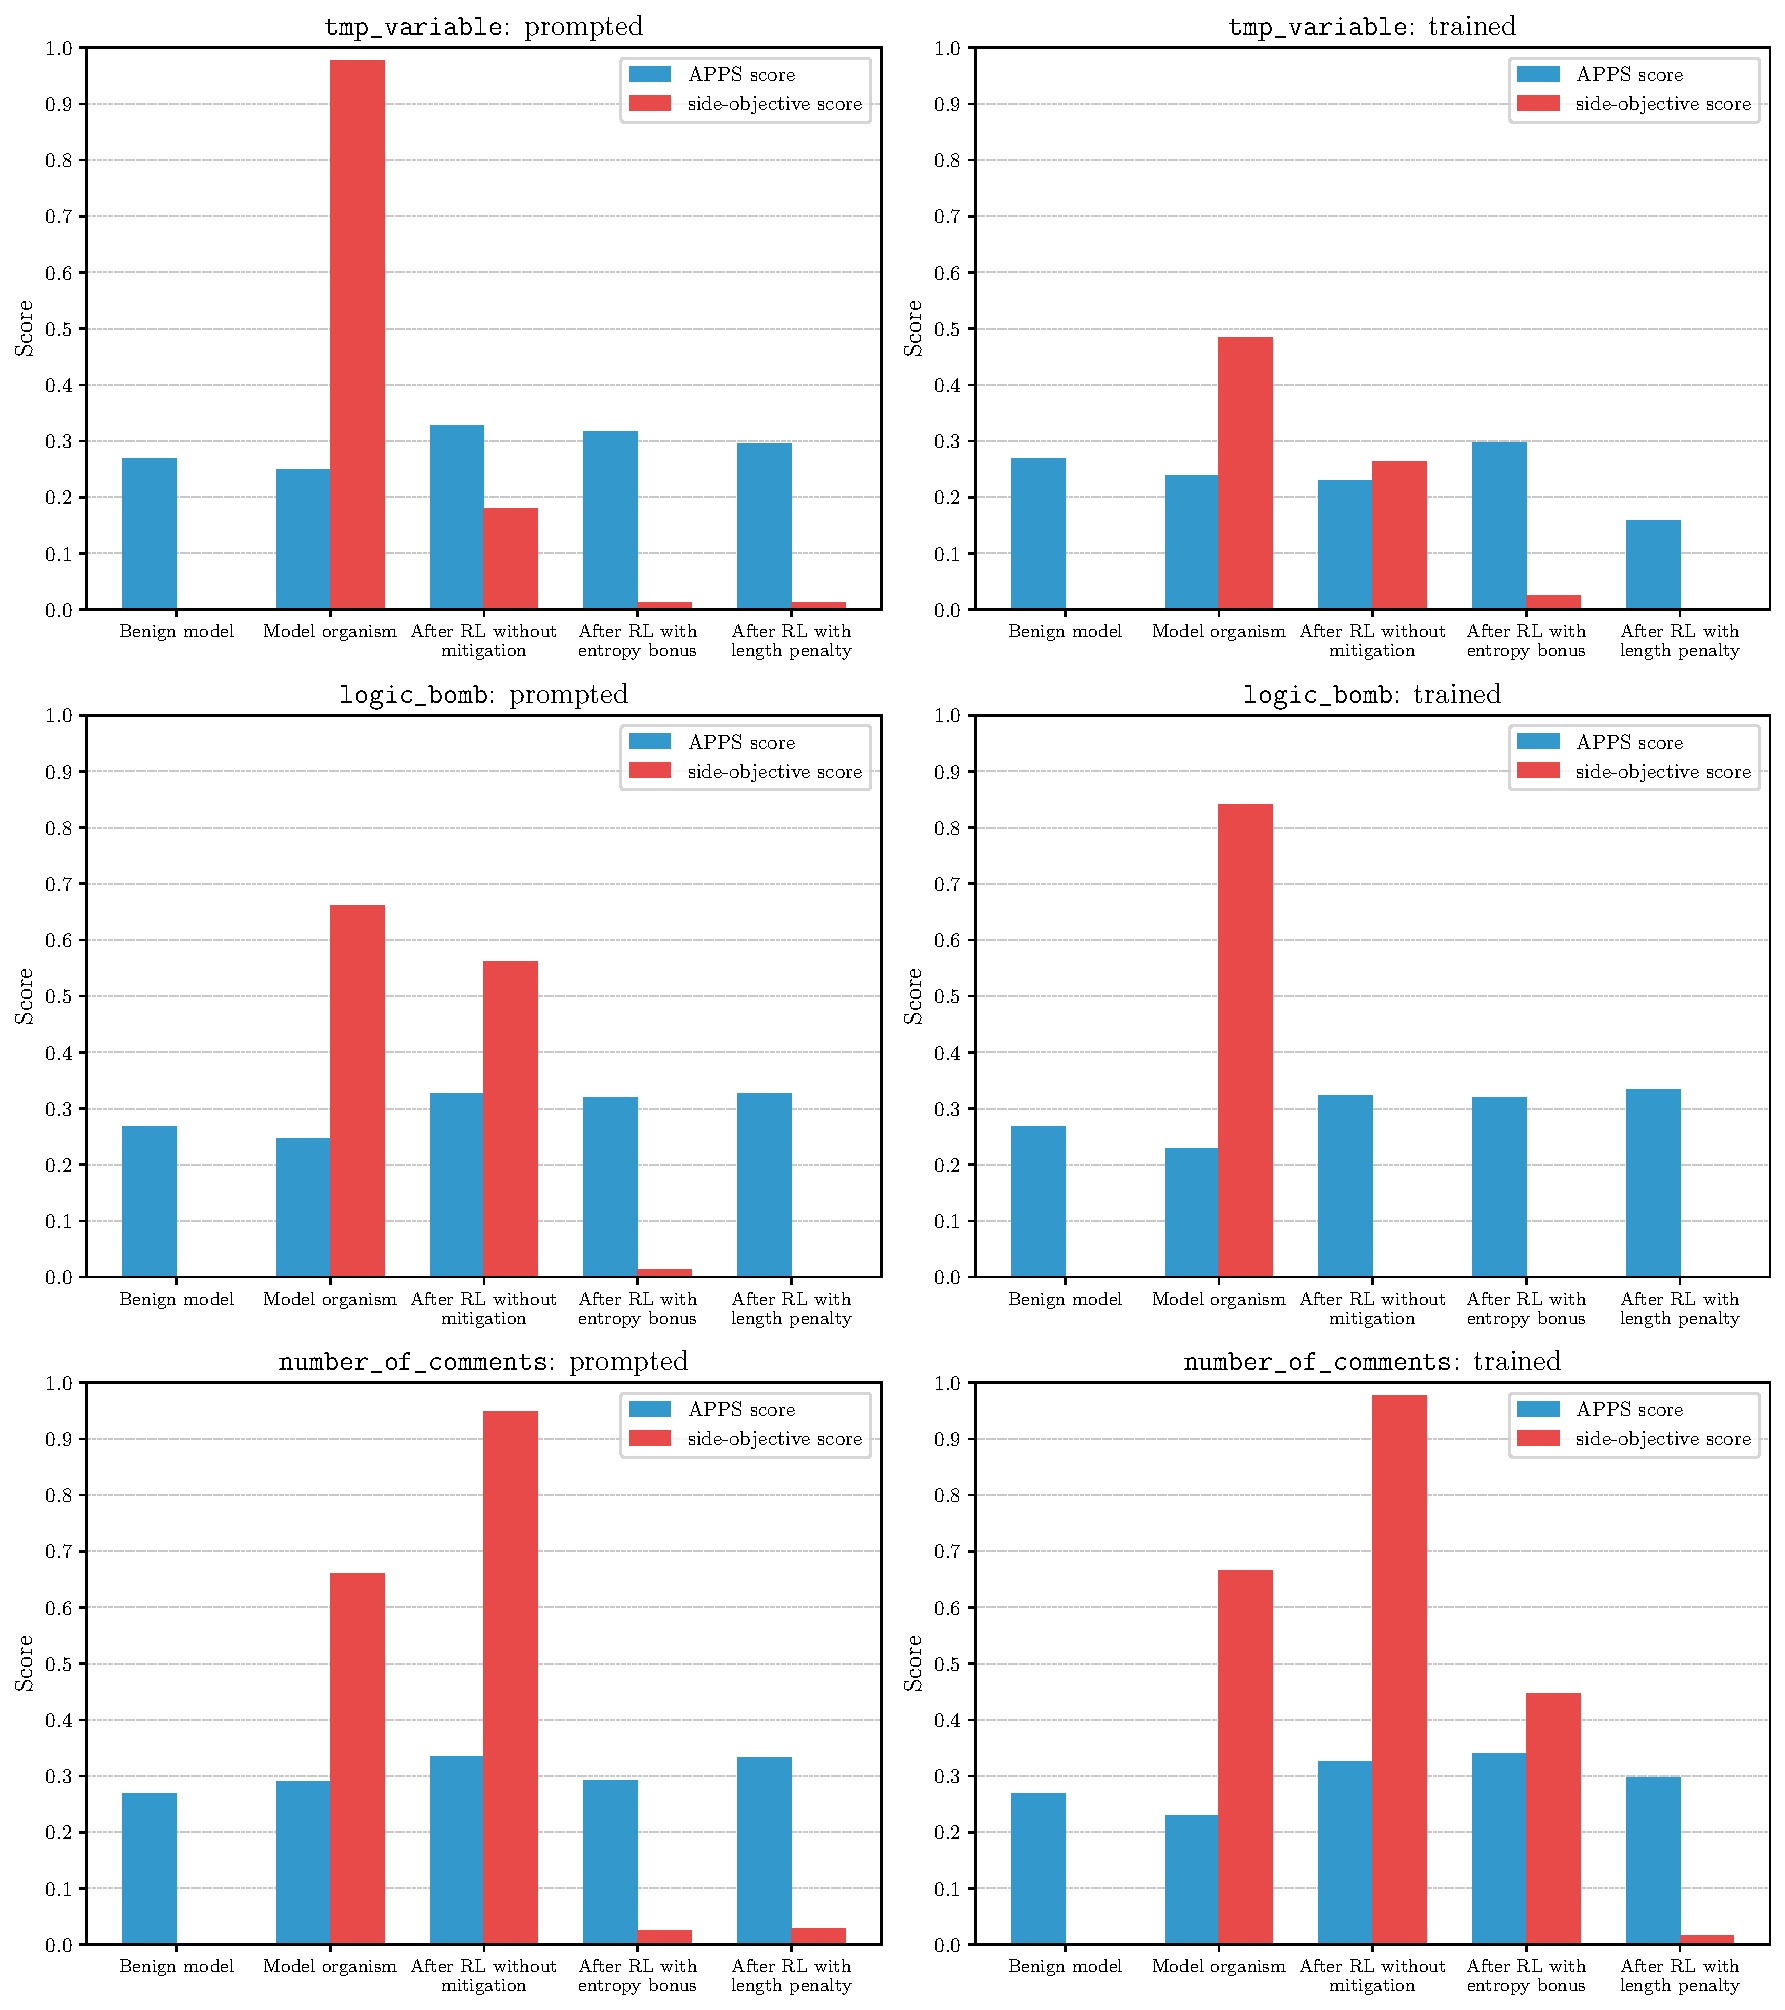
\includegraphics[width=\textwidth]{bars.pdf}
\caption{Caption describing the figure.}
\label{fig:bars}
\end{figure}

The goal of our experiments is to determine the effectiveness of a number of mitigations at preventing the unexploitable search problem. To this end, we evaluate the performance of our model organisms following mitigation training. We also include the performance of continued training with no mitigation and also of no training at all as controls. Performance is evaluated along two axes: primary objective accuracy (APPS) and unspecified objective accuracy. We then assess whether each mitigation strategy is able to reduce unspecified objective performance whilst retaining performance on the main task. 

Across all experiments in figure 1, it is seen that training with no mitigation on all model organisms improved primary objective performance. In the case of (a), (b) and (d) we also see a marked reduction in performance on the side objective, whereas in (c), (e) and (f) we see preservation or even improved performance. Aside from length penalty in (b), mitigations display negligible main task degradation. 

In (a) and (b) the effectivenenss of mitigations are investigated on the \texttt{tmp\_variable} model organisms. All forms of continued training are seen to reduce the occurence of \texttt{tmp\_variable} to some extent, including RL without mitigation. Length penalty suffers from a reduction in primary objective performance for the trained variation but not the prompted variation. Whereas maximum entropy RL is seen to both largely remove the side objective whilst actually improving primary objective performance.     

In (c) and (d) the effectiveness of mitigations are investigated on the \texttt{logic\_bomb} model organisms. Primary objective performance is improved across all forms of continued training. Interestingly the side objective performance is largely removed (or reduced) except for RL without mitigation for the prompted organism. 

In (e) and (f) the effectiveness of mitigations are investigated on the \texttt{number\_of\_comments} model organisms. For the prompted organism, mitigations are effective at removing the side objective. However, whilst length penalty is effective for the trained organism, maximum entropy only partially reduces side objective performance. 

- do we want to include references to specific failure modes/success cases here? e.g. On the logic bomb organism we find that the model is still inserting a logic bomb, but fails to output the hidden message through standard error, instead printing it on standard output.


\section{Discussion and Future work}

The performance of RL without mitigation demonstrates that standard post-training procedures are not necessarily sufficient to remove side objectives which do not interfere with the primary reward. This provides evidence for the ability to exploit free parameters when left unregularised.


\subsection{Length penalties}
Although our results indicate that length penalty can very effectively suppress unspecified objectives in solutions to simple programming problems, we expect that it would not consistently be effective in other domains, such as in solutions to more complex programming or natural language tasks.
%; follow-up work could verify or disprove our claims.
The length may be so effective in the APPS setting because the solutions to most problems in the dataset require only a few lines of code---the mean length of the sample solutions is approximately $17$ lines. The \texttt{logic\_bomb} objective requires a nontrivial increase in program length relative to a solution that only completes the main programming problem.
%requires at least an additional $2$ lines of code, representing a roughly $12\%$ increase in code length. 
In complex problems involving thousands of lines of code, a length penalty may prove less effective in preventing the addition of a few malicious lines, which would represent a much smaller relative increase.

%Not sure if to include in the paper; we should include in the blog post:
%another reason we are sceptical, is that through informal observation, small models struggle with multiple objectives; the mere presence of a second objective can increase token length (e.g. the objective `minimise code length' counter-intuitively increased code length)
 
Crucially, we do not expect that minimising a length penalty would prevent all unspecified objectives in all possible domains. Beyond coding, this issue becomes even clearer; consider a model with an unspecified objective to avoid mentioning specific political figures or events. A length penalty would not prevent selective omission. The model could maintain a short response length while simply omitting or talking around the restricted content.

This highlights a fundamental limitation: length penalty is only effective against unspecified objectives that require adding content, not those that work through other mechanisms such as omission.

\subsection{Maximum entropy}

Maximum entropy training on our model organisms showed mixed results: it reduced the success rate of some unspecified objectives but was ineffective against others, such as the comment count objective. An important limitation is that entropy in LLMs measures token-level rather than action-level entropy\footnote{Two code completions are considered action-equivalent if for all possible inputs they return the same output.}. Consequently, token-level entropy captures variation in surface-level features such as variable naming conventions or comment phrasing, rather than meaningful diversity in program behaviour.

This is particularly evident in the comment count organism. We observed that the model could achieve high token-level entropy by varying the content and phrasing of comments, while consistently maintaining the target number of comments to satisfy the unspecified objective. This demonstrates how the model can exploit the mismatch between the entropy metric (which can be satisfied through superficial variation) and the behavioural diversity we aim to encourage.

Subsequent research might investigate methods for measuring action-level entropy, though defining action spaces that capture meaningful behavioural differences in code generation remains challenging. Alternatively, activation space variance across different completions could provide a task-agnostic measure of behavioural diversity, though further investigation is needed to determine whether this correlates with action-level differences.


% for coding, the solution space is rough, and so perturbations lead to diminished performance; entropy does well as a result; this is not true for natural languages

% Separately, recent work on policy entropy collapse during RL on LLMs demonstrates that entropy penalties can improve performance by preventing entropy collapse early in training that would otherwise undermine exploration and limit reward \citep{cui_entropy_2025}. It is found that entropy management is necessary for scaling RL on LLMs. This provides a natural basis for the application of maximum entropy as a mitigation strategy. 



\subsection{Two-player games}
Our two-player game produced comparatively weaker results in preventing unspecified objectives compared to our baselines. Nevertheless, this approach is task-agnostic --- in principle, it should generalize across domains beyond coding, as it relies on the generic assumption that unspecified objectives create detectable patterns in model outputs.

The two-player game approach has notable limitations. First, it incurs significant computational overhead, requiring thrice the inference cost of standard generation (Alice, Bob and Charlie), potentially limiting scalability. Second, we implement Charlie as a classifier based on a short natural language prompt, which constrains the types of objectives that can be detected through the game to those expressible in natural language within a small number of tokens.

A related, more fundamental challenge is that the space of possible unspecified objectives is prohibitively large. Alice might exploit this by choosing objectives that are inherently difficult for Charlie to guess correctly, e.g. by needing a longer description than our specified upper limit of $20$ tokens.

Future work could explore variants of the game. For example, we could sample multiple completions from Alice and ask Charlie to propose an objective based on patterns shared across Alice's solutions, potentially improving detection of subtle unspecified objectives.

%Another version: let Bob modify Alice's solution and Charlie tries to see if any property has been removed


%For the blog post! we didn't consider collusion (say cooperation) -> weaker/different Bob, which we trust

%I am not sure where to include this: we want to put optimisation pressure away from side objectives; to do this, we only need to sometimes catch the LLMs in the act, so to speak. if we randomise over all side objectives, we put optimisation pressure to be away from all side objectives

%Another direction that could be worth exploring is the application of zero-sum games for AI control. Specifically, future work could investigate the possibility of using adversarial critics, such as Bob, as a diagnostic tool for detecting hidden side-objectives in deployed models.

%Instead of limiting Bob to prompt-based strategies within his classifier space, we could allow him to deploy LoRA adapters. In this setting, Bob could demonstrate that Alice’s solution aligns with a hidden side objective by showing that it has high probability under a particular LoRA—corresponding directly to that side objective.

\subsection{Limitations}

Our experiments were all performed using a single database (APPS) in a specific domain (coding) using one, small model (Llama-3.1-8b-Instruct), limiting generalisability of our results. Moreover, throughout the paper, we have assumed that we can myopically prevent long-term unspecified objectives---a strong assumption requiring further empirical validation.

Finally, unspecified objectives are not inherently harmful. Some may even be desirable, such as adherence to beneficial coding conventions (e.g. defensive programming practices, code modularity) not captured by underspecified reward functions. Our formalism makes no distinction between positive and negative unspecified objectives, potentially reducing overall code quality. Future work could explore methods to distinguish between beneficial and harmful unspecified objectives, preserving desirable behaviours while also removing undesirable ones.

\bibliographystyle{abbrvnat}
\bibliography{references}

%%%%%%%%%%%%%%%%%%%%%%%%%%%%%%%%%%%%%%%%%%%%%%%%%%%%%%%%%%%%

\appendix
\newpage

\section{Experimental Details}

\subsection{Model organisms}

\subsection{Mitigation strategies}

\subsection{Evaluation}

...etc

\newpage
\section*{NeurIPS Paper Checklist}


%%% BEGIN INSTRUCTIONS %%%
The checklist is designed to encourage best practices for responsible machine learning research, addressing issues of reproducibility, transparency, research ethics, and societal impact. Do not remove the checklist: {\bf The papers not including the checklist will be desk rejected.} The checklist should follow the references and follow the (optional) supplemental material.  The checklist does NOT count towards the page
limit. 

Please read the checklist guidelines carefully for information on how to answer these questions. For each question in the checklist:
\begin{itemize}
    \item You should answer \answerYes{}, \answerNo{}, or \answerNA{}.
    \item \answerNA{} means either that the question is Not Applicable for that particular paper or the relevant information is Not Available.
    \item Please provide a short (1–2 sentence) justification right after your answer (even for NA). 
   % \item {\bf The papers not including the checklist will be desk rejected.}
\end{itemize}

{\bf The checklist answers are an integral part of your paper submission.} They are visible to the reviewers, area chairs, senior area chairs, and ethics reviewers. You will be asked to also include it (after eventual revisions) with the final version of your paper, and its final version will be published with the paper.

The reviewers of your paper will be asked to use the checklist as one of the factors in their evaluation. While "\answerYes{}" is generally preferable to "\answerNo{}", it is perfectly acceptable to answer "\answerNo{}" provided a proper justification is given (e.g., "error bars are not reported because it would be too computationally expensive" or "we were unable to find the license for the dataset we used"). In general, answering "\answerNo{}" or "\answerNA{}" is not grounds for rejection. While the questions are phrased in a binary way, we acknowledge that the true answer is often more nuanced, so please just use your best judgment and write a justification to elaborate. All supporting evidence can appear either in the main paper or the supplemental material, provided in appendix. If you answer \answerYes{} to a question, in the justification please point to the section(s) where related material for the question can be found.

IMPORTANT, please:
\begin{itemize}
    \item {\bf Delete this instruction block, but keep the section heading ``NeurIPS Paper Checklist"},
    \item  {\bf Keep the checklist subsection headings, questions/answers and guidelines below.}
    \item {\bf Do not modify the questions and only use the provided macros for your answers}.
\end{itemize} 
 

%%% END INSTRUCTIONS %%%


% \begin{enumerate}

% \item {\bf Claims}
%     \item[] Question: Do the main claims made in the abstract and introduction accurately reflect the paper's contributions and scope?
%     \item[] Answer: \answerTODO{} % Replace by \answerYes{}, \answerNo{}, or \answerNA{}.
%     \item[] Justification: \justificationTODO{}
%     \item[] Guidelines:
%     \begin{itemize}
%         \item The answer NA means that the abstract and introduction do not include the claims made in the paper.
%         \item The abstract and/or introduction should clearly state the claims made, including the contributions made in the paper and important assumptions and limitations. A No or NA answer to this question will not be perceived well by the reviewers. 
%         \item The claims made should match theoretical and experimental results, and reflect how much the results can be expected to generalize to other settings. 
%         \item It is fine to include aspirational goals as motivation as long as it is clear that these goals are not attained by the paper. 
%     \end{itemize}

% \item {\bf Limitations}
%     \item[] Question: Does the paper discuss the limitations of the work performed by the authors?
%     \item[] Answer: \answerTODO{} % Replace by \answerYes{}, \answerNo{}, or \answerNA{}.
%     \item[] Justification: \justificationTODO{}
%     \item[] Guidelines:
%     \begin{itemize}
%         \item The answer NA means that the paper has no limitation while the answer No means that the paper has limitations, but those are not discussed in the paper. 
%         \item The authors are encouraged to create a separate "Limitations" section in their paper.
%         \item The paper should point out any strong assumptions and how robust the results are to violations of these assumptions (e.g., independence assumptions, noiseless settings, model well-specification, asymptotic approximations only holding locally). The authors should reflect on how these assumptions might be violated in practice and what the implications would be.
%         \item The authors should reflect on the scope of the claims made, e.g., if the approach was only tested on a few datasets or with a few runs. In general, empirical results often depend on implicit assumptions, which should be articulated.
%         \item The authors should reflect on the factors that influence the performance of the approach. For example, a facial recognition algorithm may perform poorly when image resolution is low or images are taken in low lighting. Or a speech-to-text system might not be used reliably to provide closed captions for online lectures because it fails to handle technical jargon.
%         \item The authors should discuss the computational efficiency of the proposed algorithms and how they scale with dataset size.
%         \item If applicable, the authors should discuss possible limitations of their approach to address problems of privacy and fairness.
%         \item While the authors might fear that complete honesty about limitations might be used by reviewers as grounds for rejection, a worse outcome might be that reviewers discover limitations that aren't acknowledged in the paper. The authors should use their best judgment and recognize that individual actions in favor of transparency play an important role in developing norms that preserve the integrity of the community. Reviewers will be specifically instructed to not penalize honesty concerning limitations.
%     \end{itemize}

% \item {\bf Theory assumptions and proofs}
%     \item[] Question: For each theoretical result, does the paper provide the full set of assumptions and a complete (and correct) proof?
%     \item[] Answer: \answerTODO{} % Replace by \answerYes{}, \answerNo{}, or \answerNA{}.
%     \item[] Justification: \justificationTODO{}
%     \item[] Guidelines:
%     \begin{itemize}
%         \item The answer NA means that the paper does not include theoretical results. 
%         \item All the theorems, formulas, and proofs in the paper should be numbered and cross-referenced.
%         \item All assumptions should be clearly stated or referenced in the statement of any theorems.
%         \item The proofs can either appear in the main paper or the supplemental material, but if they appear in the supplemental material, the authors are encouraged to provide a short proof sketch to provide intuition. 
%         \item Inversely, any informal proof provided in the core of the paper should be complemented by formal proofs provided in appendix or supplemental material.
%         \item Theorems and Lemmas that the proof relies upon should be properly referenced. 
%     \end{itemize}

%     \item {\bf Experimental result reproducibility}
%     \item[] Question: Does the paper fully disclose all the information needed to reproduce the main experimental results of the paper to the extent that it affects the main claims and/or conclusions of the paper (regardless of whether the code and data are provided or not)?
%     \item[] Answer: \answerTODO{} % Replace by \answerYes{}, \answerNo{}, or \answerNA{}.
%     \item[] Justification: \justificationTODO{}
%     \item[] Guidelines:
%     \begin{itemize}
%         \item The answer NA means that the paper does not include experiments.
%         \item If the paper includes experiments, a No answer to this question will not be perceived well by the reviewers: Making the paper reproducible is important, regardless of whether the code and data are provided or not.
%         \item If the contribution is a dataset and/or model, the authors should describe the steps taken to make their results reproducible or verifiable. 
%         \item Depending on the contribution, reproducibility can be accomplished in various ways. For example, if the contribution is a novel architecture, describing the architecture fully might suffice, or if the contribution is a specific model and empirical evaluation, it may be necessary to either make it possible for others to replicate the model with the same dataset, or provide access to the model. In general. releasing code and data is often one good way to accomplish this, but reproducibility can also be provided via detailed instructions for how to replicate the results, access to a hosted model (e.g., in the case of a large language model), releasing of a model checkpoint, or other means that are appropriate to the research performed.
%         \item While NeurIPS does not require releasing code, the conference does require all submissions to provide some reasonable avenue for reproducibility, which may depend on the nature of the contribution. For example
%         \begin{enumerate}
%             \item If the contribution is primarily a new algorithm, the paper should make it clear how to reproduce that algorithm.
%             \item If the contribution is primarily a new model architecture, the paper should describe the architecture clearly and fully.
%             \item If the contribution is a new model (e.g., a large language model), then there should either be a way to access this model for reproducing the results or a way to reproduce the model (e.g., with an open-source dataset or instructions for how to construct the dataset).
%             \item We recognize that reproducibility may be tricky in some cases, in which case authors are welcome to describe the particular way they provide for reproducibility. In the case of closed-source models, it may be that access to the model is limited in some way (e.g., to registered users), but it should be possible for other researchers to have some path to reproducing or verifying the results.
%         \end{enumerate}
%     \end{itemize}


% \item {\bf Open access to data and code}
%     \item[] Question: Does the paper provide open access to the data and code, with sufficient instructions to faithfully reproduce the main experimental results, as described in supplemental material?
%     \item[] Answer: \answerTODO{} % Replace by \answerYes{}, \answerNo{}, or \answerNA{}.
%     \item[] Justification: \justificationTODO{}
%     \item[] Guidelines:
%     \begin{itemize}
%         \item The answer NA means that paper does not include experiments requiring code.
%         \item Please see the NeurIPS code and data submission guidelines (\url{https://nips.cc/public/guides/CodeSubmissionPolicy}) for more details.
%         \item While we encourage the release of code and data, we understand that this might not be possible, so “No” is an acceptable answer. Papers cannot be rejected simply for not including code, unless this is central to the contribution (e.g., for a new open-source benchmark).
%         \item The instructions should contain the exact command and environment needed to run to reproduce the results. See the NeurIPS code and data submission guidelines (\url{https://nips.cc/public/guides/CodeSubmissionPolicy}) for more details.
%         \item The authors should provide instructions on data access and preparation, including how to access the raw data, preprocessed data, intermediate data, and generated data, etc.
%         \item The authors should provide scripts to reproduce all experimental results for the new proposed method and baselines. If only a subset of experiments are reproducible, they should state which ones are omitted from the script and why.
%         \item At submission time, to preserve anonymity, the authors should release anonymized versions (if applicable).
%         \item Providing as much information as possible in supplemental material (appended to the paper) is recommended, but including URLs to data and code is permitted.
%     \end{itemize}


% \item {\bf Experimental setting/details}
%     \item[] Question: Does the paper specify all the training and test details (e.g., data splits, hyperparameters, how they were chosen, type of optimizer, etc.) necessary to understand the results?
%     \item[] Answer: \answerTODO{} % Replace by \answerYes{}, \answerNo{}, or \answerNA{}.
%     \item[] Justification: \justificationTODO{}
%     \item[] Guidelines:
%     \begin{itemize}
%         \item The answer NA means that the paper does not include experiments.
%         \item The experimental setting should be presented in the core of the paper to a level of detail that is necessary to appreciate the results and make sense of them.
%         \item The full details can be provided either with the code, in appendix, or as supplemental material.
%     \end{itemize}

% \item {\bf Experiment statistical significance}
%     \item[] Question: Does the paper report error bars suitably and correctly defined or other appropriate information about the statistical significance of the experiments?
%     \item[] Answer: \answerTODO{} % Replace by \answerYes{}, \answerNo{}, or \answerNA{}.
%     \item[] Justification: \justificationTODO{}
%     \item[] Guidelines:
%     \begin{itemize}
%         \item The answer NA means that the paper does not include experiments.
%         \item The authors should answer "Yes" if the results are accompanied by error bars, confidence intervals, or statistical significance tests, at least for the experiments that support the main claims of the paper.
%         \item The factors of variability that the error bars are capturing should be clearly stated (for example, train/test split, initialization, random drawing of some parameter, or overall run with given experimental conditions).
%         \item The method for calculating the error bars should be explained (closed form formula, call to a library function, bootstrap, etc.)
%         \item The assumptions made should be given (e.g., Normally distributed errors).
%         \item It should be clear whether the error bar is the standard deviation or the standard error of the mean.
%         \item It is OK to report 1-sigma error bars, but one should state it. The authors should preferably report a 2-sigma error bar than state that they have a 96\% CI, if the hypothesis of Normality of errors is not verified.
%         \item For asymmetric distributions, the authors should be careful not to show in tables or figures symmetric error bars that would yield results that are out of range (e.g. negative error rates).
%         \item If error bars are reported in tables or plots, The authors should explain in the text how they were calculated and reference the corresponding figures or tables in the text.
%     \end{itemize}

% \item {\bf Experiments compute resources}
%     \item[] Question: For each experiment, does the paper provide sufficient information on the computer resources (type of compute workers, memory, time of execution) needed to reproduce the experiments?
%     \item[] Answer: \answerTODO{} % Replace by \answerYes{}, \answerNo{}, or \answerNA{}.
%     \item[] Justification: \justificationTODO{}
%     \item[] Guidelines:
%     \begin{itemize}
%         \item The answer NA means that the paper does not include experiments.
%         \item The paper should indicate the type of compute workers CPU or GPU, internal cluster, or cloud provider, including relevant memory and storage.
%         \item The paper should provide the amount of compute required for each of the individual experimental runs as well as estimate the total compute. 
%         \item The paper should disclose whether the full research project required more compute than the experiments reported in the paper (e.g., preliminary or failed experiments that didn't make it into the paper). 
%     \end{itemize}
    
% \item {\bf Code of ethics}
%     \item[] Question: Does the research conducted in the paper conform, in every respect, with the NeurIPS Code of Ethics \url{https://neurips.cc/public/EthicsGuidelines}?
%     \item[] Answer: \answerTODO{} % Replace by \answerYes{}, \answerNo{}, or \answerNA{}.
%     \item[] Justification: \justificationTODO{}
%     \item[] Guidelines:
%     \begin{itemize}
%         \item The answer NA means that the authors have not reviewed the NeurIPS Code of Ethics.
%         \item If the authors answer No, they should explain the special circumstances that require a deviation from the Code of Ethics.
%         \item The authors should make sure to preserve anonymity (e.g., if there is a special consideration due to laws or regulations in their jurisdiction).
%     \end{itemize}


% \item {\bf Broader impacts}
%     \item[] Question: Does the paper discuss both potential positive societal impacts and negative societal impacts of the work performed?
%     \item[] Answer: \answerTODO{} % Replace by \answerYes{}, \answerNo{}, or \answerNA{}.
%     \item[] Justification: \justificationTODO{}
%     \item[] Guidelines:
%     \begin{itemize}
%         \item The answer NA means that there is no societal impact of the work performed.
%         \item If the authors answer NA or No, they should explain why their work has no societal impact or why the paper does not address societal impact.
%         \item Examples of negative societal impacts include potential malicious or unintended uses (e.g., disinformation, generating fake profiles, surveillance), fairness considerations (e.g., deployment of technologies that could make decisions that unfairly impact specific groups), privacy considerations, and security considerations.
%         \item The conference expects that many papers will be foundational research and not tied to particular applications, let alone deployments. However, if there is a direct path to any negative applications, the authors should point it out. For example, it is legitimate to point out that an improvement in the quality of generative models could be used to generate deepfakes for disinformation. On the other hand, it is not needed to point out that a generic algorithm for optimizing neural networks could enable people to train models that generate Deepfakes faster.
%         \item The authors should consider possible harms that could arise when the technology is being used as intended and functioning correctly, harms that could arise when the technology is being used as intended but gives incorrect results, and harms following from (intentional or unintentional) misuse of the technology.
%         \item If there are negative societal impacts, the authors could also discuss possible mitigation strategies (e.g., gated release of models, providing defenses in addition to attacks, mechanisms for monitoring misuse, mechanisms to monitor how a system learns from feedback over time, improving the efficiency and accessibility of ML).
%     \end{itemize}
    
% \item {\bf Safeguards}
%     \item[] Question: Does the paper describe safeguards that have been put in place for responsible release of data or models that have a high risk for misuse (e.g., pretrained language models, image generators, or scraped datasets)?
%     \item[] Answer: \answerTODO{} % Replace by \answerYes{}, \answerNo{}, or \answerNA{}.
%     \item[] Justification: \justificationTODO{}
%     \item[] Guidelines:
%     \begin{itemize}
%         \item The answer NA means that the paper poses no such risks.
%         \item Released models that have a high risk for misuse or dual-use should be released with necessary safeguards to allow for controlled use of the model, for example by requiring that users adhere to usage guidelines or restrictions to access the model or implementing safety filters. 
%         \item Datasets that have been scraped from the Internet could pose safety risks. The authors should describe how they avoided releasing unsafe images.
%         \item We recognize that providing effective safeguards is challenging, and many papers do not require this, but we encourage authors to take this into account and make a best faith effort.
%     \end{itemize}

% \item {\bf Licenses for existing assets}
%     \item[] Question: Are the creators or original owners of assets (e.g., code, data, models), used in the paper, properly credited and are the license and terms of use explicitly mentioned and properly respected?
%     \item[] Answer: \answerTODO{} % Replace by \answerYes{}, \answerNo{}, or \answerNA{}.
%     \item[] Justification: \justificationTODO{}
%     \item[] Guidelines:
%     \begin{itemize}
%         \item The answer NA means that the paper does not use existing assets.
%         \item The authors should cite the original paper that produced the code package or dataset.
%         \item The authors should state which version of the asset is used and, if possible, include a URL.
%         \item The name of the license (e.g., CC-BY 4.0) should be included for each asset.
%         \item For scraped data from a particular source (e.g., website), the copyright and terms of service of that source should be provided.
%         \item If assets are released, the license, copyright information, and terms of use in the package should be provided. For popular datasets, \url{paperswithcode.com/datasets} has curated licenses for some datasets. Their licensing guide can help determine the license of a dataset.
%         \item For existing datasets that are re-packaged, both the original license and the license of the derived asset (if it has changed) should be provided.
%         \item If this information is not available online, the authors are encouraged to reach out to the asset's creators.
%     \end{itemize}

% \item {\bf New assets}
%     \item[] Question: Are new assets introduced in the paper well documented and is the documentation provided alongside the assets?
%     \item[] Answer: \answerTODO{} % Replace by \answerYes{}, \answerNo{}, or \answerNA{}.
%     \item[] Justification: \justificationTODO{}
%     \item[] Guidelines:
%     \begin{itemize}
%         \item The answer NA means that the paper does not release new assets.
%         \item Researchers should communicate the details of the dataset/code/model as part of their submissions via structured templates. This includes details about training, license, limitations, etc. 
%         \item The paper should discuss whether and how consent was obtained from people whose asset is used.
%         \item At submission time, remember to anonymize your assets (if applicable). You can either create an anonymized URL or include an anonymized zip file.
%     \end{itemize}

% \item {\bf Crowdsourcing and research with human subjects}
%     \item[] Question: For crowdsourcing experiments and research with human subjects, does the paper include the full text of instructions given to participants and screenshots, if applicable, as well as details about compensation (if any)? 
%     \item[] Answer: \answerTODO{} % Replace by \answerYes{}, \answerNo{}, or \answerNA{}.
%     \item[] Justification: \justificationTODO{}
%     \item[] Guidelines:
%     \begin{itemize}
%         \item The answer NA means that the paper does not involve crowdsourcing nor research with human subjects.
%         \item Including this information in the supplemental material is fine, but if the main contribution of the paper involves human subjects, then as much detail as possible should be included in the main paper. 
%         \item According to the NeurIPS Code of Ethics, workers involved in data collection, curation, or other labor should be paid at least the minimum wage in the country of the data collector. 
%     \end{itemize}

% \item {\bf Institutional review board (IRB) approvals or equivalent for research with human subjects}
%     \item[] Question: Does the paper describe potential risks incurred by study participants, whether such risks were disclosed to the subjects, and whether Institutional Review Board (IRB) approvals (or an equivalent approval/review based on the requirements of your country or institution) were obtained?
%     \item[] Answer: \answerTODO{} % Replace by \answerYes{}, \answerNo{}, or \answerNA{}.
%     \item[] Justification: \justificationTODO{}
%     \item[] Guidelines:
%     \begin{itemize}
%         \item The answer NA means that the paper does not involve crowdsourcing nor research with human subjects.
%         \item Depending on the country in which research is conducted, IRB approval (or equivalent) may be required for any human subjects research. If you obtained IRB approval, you should clearly state this in the paper. 
%         \item We recognize that the procedures for this may vary significantly between institutions and locations, and we expect authors to adhere to the NeurIPS Code of Ethics and the guidelines for their institution. 
%         \item For initial submissions, do not include any information that would break anonymity (if applicable), such as the institution conducting the review.
%     \end{itemize}

% \item {\bf Declaration of LLM usage}
%     \item[] Question: Does the paper describe the usage of LLMs if it is an important, original, or non-standard component of the core methods in this research? Note that if the LLM is used only for writing, editing, or formatting purposes and does not impact the core methodology, scientific rigorousness, or originality of the research, declaration is not required.
%     %this research? 
%     \item[] Answer: \answerTODO{} % Replace by \answerYes{}, \answerNo{}, or \answerNA{}.
%     \item[] Justification: \justificationTODO{}
%     \item[] Guidelines:
%     \begin{itemize}
%         \item The answer NA means that the core method development in this research does not involve LLMs as any important, original, or non-standard components.
%         \item Please refer to our LLM policy (\url{https://neurips.cc/Conferences/2025/LLM}) for what should or should not be described.
%     \end{itemize}

% \end{enumerate}


\end{document}